\chapter{環境変数}
この章では,環境変数について学ぶ.
環境変数はシェルが管理する変数である.
変数とはいえC言語の変数とは全く別の仕組みである.
環境変数はシェルから,シェルによって起動されたプロセスにコピーされる.
プロセス(プログラム)は実行時に環境変数の値を調べることができる.
例えば,使用言語を表す環境変数を参照しエラーメッセージの言語を
切り替えるようにプログラムを作っておけば,
一種類のプログラムを世界中で使うことができる.

%==============================================================================
\section{環境変数と使用例}
リスト\ref{environmentVariableSample}に
macOSやUNIXでよく使用される環境変数の「名前」と「値」の例を示す.

\lstinputlisting[numbers=none,caption=よく使用される環境変数,
  label=environmentVariableSample,float=btp]{Lst/environmentVariableSample.txt}

例えば\texttt{LC\_TIME}環境変数は日時の表示に使用する言語を決める.
また,\texttt{TZ}環境変数はどの地域の時刻を表示するか決める.
date コマンド(現在時刻表示),cal コマンド(カレンダー表示),
ls コマンド(ファイルの最終変更時刻表示)等がこれらの環境変数の値により
日時の表示を変化させる.

リスト\ref{environmentVariableLCTIME}に,
これら環境変数の値を変化しながらコマンドを実行した例を示す.
例えばdateコマンドは現在時刻を,
\texttt{LC\_TIME}環境変数の値が\texttt{C}なら英語表記で表示するが,
\texttt{ja\_JP.UTF-8}なら日本語表記で表示する.
\texttt{TZ}環境変数の値が\texttt{Japan}なら日本時間で表示するが,
\texttt{Cuba}ならキューバ時間で表示する.
このように環境変数はプログラムの振る舞いに影響を与える.

\lstinputlisting[numbers=none,caption=環境変数の変化が与える影響の例,
  float=btp,label=environmentVariableLCTIME]{Lst/environmentVariableLCTIME.txt}

%==============================================================================
\section{環境変数を誰が決めるか}

\begin{enumerate}
\item システム管理者 \\
  システム管理者はユーザがログインした時の初期状態を決める.
  UNIXやmacOSでは,\|/etc/profile|ファイル等に書かれたスクリプトが
  全ユーザのシェル起動時に実行される.
  システム管理者は全ユーザに共通のシェルの初期化処理をここに書いておく.
  このスクリプトで全ユーザに共通の環境変数の初期化ができる.
\item ユーザの設定ファイル \\
  ユーザは自分のホームディレクトリの\|.bash_profile|ファイルに
  自分専用の初期化処理を書くことができる.
  ここに,\ref{environmentVariableOperation}で説明するコマンドを
  用いてスクリプトを書いておく.
  以下に\|.bash_profile|ファイルの例を示す\footnote{
    代入(\texttt{=})の左右に空白を書いてはならない.
    以降の書式や実行例でも同様である.}.
  \lstinputlisting[numbers=none]{Lst/dotBashRc.txt}
\item ユーザによるコマンド操作 \\
  シェルのコマンド操作で環境変数を操作することができる.
  但し,影響範囲は操作したウインドのシェルのみである.
  また,次回のログイン時には操作結果の影響は残らない.
\end{enumerate}

%==============================================================================
\section{環境変数の操作}\label{environmentVariableOperation}
以下では,コマンドラインで環境変数を操作する方法を解説する.

\subsection{表示}
printenv コマンドを用いて環境変数を表示する.

\begin{description}
\item[書式] \texttt{name}は環境変数の名前である.
\begin{lstlisting}[numbers=none]
  printenv [name]
\end{lstlisting}
\item[解説]
  \texttt{name} を省略した場合は,
  全ての環境変数の名前と値を表示する.
  \texttt{name} を書いた場合は該当のする環境変数の\emph{値だけ}表示する.
  該当する環境変数が無い場合は何も表示しない.
\item [実行例]  macOS 上での printenvコマンドの実行例を示す.
  環境変数の名前を省略して実行した場合は,
  全ての環境変数について「名前=値」形式で表示される.
  \lstinputlisting[numbers=none]{Lst/environmentVariablePrintenv.txt}
\end{description}

\subsection{新規作成(その1)}
UNIXの標準シェル(sh)での操作方法を説明する.

\begin{description}
\item[書式] 次の2ステップで操作を行う.
\begin{lstlisting}
  name=value
  export name
\end{lstlisting}
\item[解説]
  1行で,一旦,シェル変数を作る.
  2行でシェル変数を環境変数に変更する.
\item[実行例]
  1行は\texttt{MYNAME}環境変数が存在するか確認している.
  \texttt{MYNAME}環境変数は存在しないので何も表示されない.
  2,3行で値が\texttt{sigemura}の\texttt{MYNAME}環境変数を作った.
  4行で\texttt{MYNAME}環境変数を確認すると
  値が\texttt{sigemura}になっていることが分かる.
  \lstinputlisting[numbers=left]{Lst/environmentVariableSh.txt}
\end{description}

\subsection{新規作成(その2)}
macOSやLinuxで使用されるシェル(bash)では,
次のように1行の操作で環境変数を作ることができる.

\begin{description}
\item[書式]
  次の1ステップで環境変数を作ることができる.
\begin{lstlisting}[numbers=none]
  export name=value
\end{lstlisting}
\item[解説]
  一旦,シェル変数を作ることなく環境変数を作ることができる.
\item[実行例]
  次のように動作確認ができる.
  \lstinputlisting[numbers=none]{Lst/environmentVariableBash.txt}
\end{description}

\subsection{値の変更}
既に存在する環境変数の値を変更することができる.

\begin{description}
\item [書式]
  \texttt{name}は環境変数の名前,\texttt{value}は新しい値である.
\begin{lstlisting}[numbers=none]
  name=value
\end{lstlisting}
\item [解説]
  「環境変数の変更」と「シェル変数の作成」は書式だけでは区別が付かない.
  変数名を間違った場合,
  間違った名前で新しいシェル変数が作成されエラーにならないので
  注意が必要である.
\item [実行例]
  \texttt{MYNAME}環境変数が既に存在している場合の実行例を示す.
  \lstinputlisting[numbers=none]{Lst/environmentVariableOverWrite.txt}
\end{description}

\subsection{値の参照}
環境変数やシェル変数の値を利用することができる.

\begin{description}
\item [書式]
  \texttt{name}は環境変数の名前である.
\begin{lstlisting}[numbers=none]
  $name
\end{lstlisting} %$
\item [解説]
  \texttt{\$name}は,
  シェルが入力されたコマンドの意味を評価する際に,
  変数の値に置き換えられる.
\item [実行例1]
  すでにある\texttt{PATH}環境変数の値に新規ディレクトリを追加する\footnote{
    システムが決めたディレクトリに,
    ユーザがディレクトリを追加することはよくある.
  }例を示す.
  \lstinputlisting[numbers=none]{Lst/environmentVariableReference.txt}
\item [実行例2]
  環境変数\texttt{i}の値を数値と見做してインクリメント\footnote{
    \texttt{expr}コマンドとsh(bash)のコマンド置換を使用している.
  }する例を示す.
  \texttt{printenv i}の代わりに\texttt{echo \$i}でも値を表示できる.
  \lstinputlisting[numbers=none]{Lst/environmentVariableIncrement.txt}
\end{description}

\subsection{変数の削除}
unsetコマンドを用いて,
環境変数やシェル変数を削除することができる.

\begin{description}
\item [書式]
  \texttt{name}は変数の名前である.
\begin{lstlisting}[numbers=none]
  unset name
\end{lstlisting}
\item [解説]
  存在しない変数を\texttt{unset}してもエラーにならない.
  変数名を間違ってもエラーにならないので注意が必要である.
\item [実行例]
  \texttt{MYNAME}環境変数が既に存在している場合の実行例を示す.
  \lstinputlisting[numbers=none]{Lst/environmentVariableUnset.txt}
\end{description}

\subsection{一時的な作成と値の変更}
env コマンドを用いて,
環境変数の値を一時的(今回のコマンド実行の期間だけ)に
変更してコマンド(プログラム)を実行したり,
一時的に環境変数を作ってコマンドを実行したりすることができる.

\begin{description}
\item [書式]
  変数へ値を代入する指示が続いた後に,実行するコマンドが続く.
\begin{lstlisting}[numbers=none]
  env name1=value1 name2=value2 ... command
\end{lstlisting}
\item [解説]
  env コマンドは代入形式のコマンド行引数が続く間,
  それらを環境変数の変更(作成)指示とみなし処理する.
  代入形式ではないコマンド行引数を見つけたら,
  それ以降を実行すべきコマンドとみなす.
\item [実行例]
  ロケール\footnote{
    囲み記事「ロケール」を参照のこと.
  }とタイムゾーン\footnote{
    囲み記事「タイムゾーン」を参照のこと.
  }を変更してdateコマンドを実行する例である.
  日時表示用のロケールを格納する\texttt{LC\_TIME}変数を日本語表示を示す値に,
  タイムゾーンを格納する\texttt{TZ}変数をキューバ時間を表す値に変更した上で,
  dateコマンドを実行している.
  その後でdateコマンドをもう一度実行し,
  環境変数の変更が一時的であることを確認している.
  \lstinputlisting[numbers=none]{Lst/environmentVariableEnv.txt}
\end{description}

\begin{figure}[btp]
\begin{itembox}[l]{ロケール}
\texttt{LANG}環境変数や\texttt{LC\_TIME}環境変数に
セットする値をロケール名と呼ぶ.
ロケール名は「言語コード」,「国名コード」と「エンコーディング」の
組み合わせで表現される.

\begin{itemize}
\item
  言語コード\footnote{
  言語コードは\url{https://ja.wikipedia.org/wiki/ISO_639-1}等を参照のこと.
  }はISO639で定義された2文字コードである(日本語は"ja").
\item 
  国名コード\footnote{
    国名コードは\url{https://ja.wikipedia.org/wiki/ISO_3166-1}等を参照のこと.
  }はISO3166で定義された2文字コードである(日本は"JP").
\item
  エンコーディングは,使用する文字符号化方式を示す.
  エンコーディングがターミナルエミュレータの
  テキストエンコーディングと一致していないと文字化けを起こす
  (macOSではUTF-8方式が使用される.).
\end{itemize}

使用可能なロケールの一覧は\|locale -a|コマンドで表示できる.
通常,macOSで日本語を使用する場合のロケール名は,
言語コード=\texttt{ja},国名コード=\texttt{JP},エンコーディング=\texttt{UTF-8}を
組み合わせて次のようになる.

\centerline{\texttt{ja\_JP.UTF-8 }(日本語\_日本.UTF-8)}
\end{itembox}
\end{figure}

\begin{figure}[btp]
\begin{itembox}[l]{タイムゾーン}
\texttt{TZ}環境変数にタイムゾーンを表す値をセットする.
macOSやUNIXの内部で時刻は協定世界時(UTC)で管理されており,
時刻を表示する時に現地時間に変換して表示する.
時刻に関係するプログラムは
協定世界時と現地時間の変換方法を\texttt{TZ}環境変数から知ることができる.
日本の場合はタイムゾーン名が\texttt{JST},協定世界時との時差が$-9$時間なので,
\|TZ=JST-9|となる.

この形式の他に\|/usr/share/zoneinfo/|に置いてあるファイル名で
タイムゾーンを指定することもできる.
\|/usr/share/zoneinfo/Cuba|ファイルが存在するので
\|TZ=Cuba|と指定できる.
\|/usr/share/zoneinfo/Japan|ファイルも存在するので
\|TZ=Japan|も指定できる.
\|/usr/share/zoneinfo/Asia/Tokyo|ファイルが存在するので
\|TZ=Asia/Tokyo|と指定しても良い.

なお,\texttt{TZ}環境変数が定義されていない時は,
OSのインストール時に選択した標準のタイムゾーンが用いられる.
\end{itembox}
\end{figure}

\newpage

%==============================================================================
\section*{課題 No.7}
\begin{enumerate}
\item ここまでの実行例を試してみなさい.
\item 囲み記事を参考に,
  \texttt{LC\_TIME}環境変数や\texttt{TZ}環境変数を変更し,
  効果を確認する.
  例えば,
  「モスクワ時間,ロシア語表記」で現在時刻を表示するにはどうしたらよいか?
\end{enumerate}
\newpage
%==============================================================================
\section{環境変数の仕組み}
環境変数を管理する仕組みと,
環境変数をプロセス間で引き継ぐ仕組みを学ぶ.

\subsection{シェルによる管理}
シェルもプログラムの一種なので,
\figref{proc}に示したようなプロセスとして実行される.
\figref{environmentVariableShell}は,
\figref{proc}をシェルプロセスの場合に当てはめた図である.
シェルプロセス(shellプロセス)は
環境変数を自プロセスのデータ領域に\footnote{
本当はスタック領域も使っているかも知れない.}記憶している.
ユーザが\|export|や\|unset|等のコマンドを入力すると,
シェルプログラムのインタプリタが意味を解釈し環境変数を操作する.
なお,
\|export|や\|unset|のような,
シェル自身によって処理されるコマンドを\emph{内部コマンド}と呼ぶ.

\begin{myfig}{btp}{環境変数をシェルの内部で管理}{environmentVariableShell}
  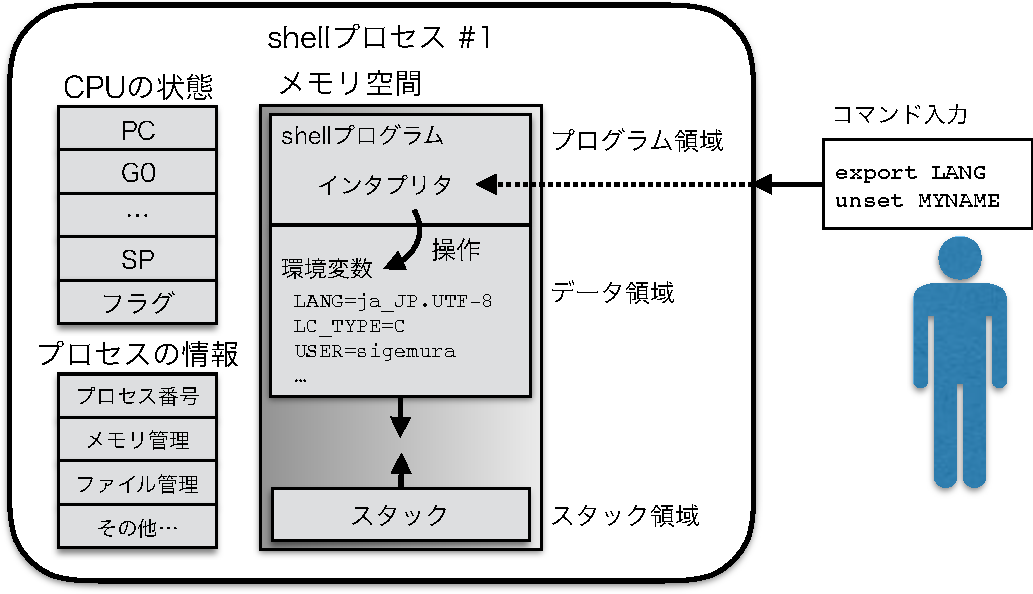
\includegraphics[scale=0.70]{Fig/environmentVariableShell-crop.pdf}
\end{myfig}

\subsection{プロセスへのコピー}
\figref{environmentVariableCopy}に示すように,
シェルは入力されたコマンドが内部コマンド以外(\emph{外部コマンド})なら,
コマンド名と同じ名前のプログラムを探し子プロセスとして起動する.
この時シェルは,
自身の環境変数を子プロセスにコピーするようにOSカーネルに依頼する.
OSカーネルは子プロセスのメモリ空間のどこか(例えばスタックの底)に
環境変数をコピーする.
子プロセスは,
自身のメモリ空間にコピーされた環境変数を,
参照・変更・削除できる.

\begin{myfig}{btp}{プログラム起動時の環境変数コピー}{environmentVariableCopy}
  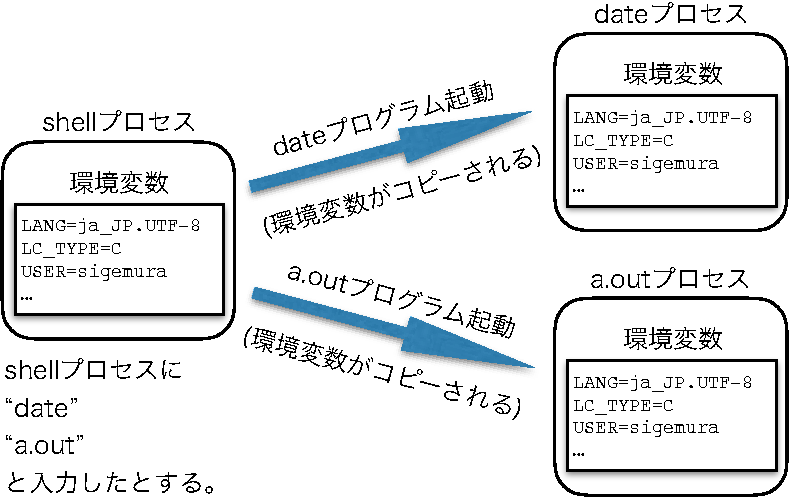
\includegraphics[scale=0.75]{Fig/environmentVariableCopy-crop.pdf}
\end{myfig}

\subsection{変更した上でのコピー}
プロセスへ環境変数をコピーする仕組みは,
シェルに限らず全ての他のプログラムを起動するプログラムで共通に用いられる.
\ref{environmentVariableOperation}で紹介したenvコマンドも,
この仕組を利用している.

envコマンドは\emph{外部コマンド}である.
envコマンドは他のプログラムを起動するプログラムとして実装できる.
\figref{environmentVariableEnv}にenvコマンドの仕組みを示す.
envコマンドは自身の環境変数を変更した後,
目的のプログラムを起動する.
その時,新しいプログラムに変更後の環境変数がコピーされる.

\begin{myfig}{btp}{env プログラムの仕組み}{environmentVariableEnv}
  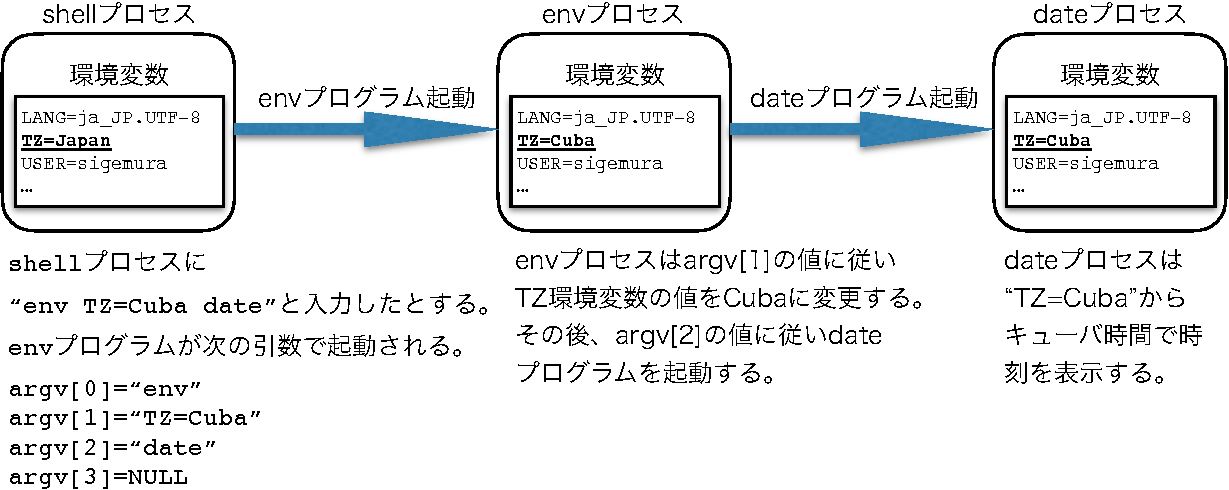
\includegraphics[scale=0.8]{Fig/environmentVariableEnv-crop.pdf}
\end{myfig}

%==============================================================================
\section{プログラムからの環境変数アクセス}
C言語プログラムから環境変数をアクセスする方法を紹介する.

\subsection{読み出し}
C言語から環境変数を読み出すために,
以下に紹介する二つの方法が使用できる.

\begin{enumerate}
\item \emph{\texttt{main}関数の\texttt{envp}仮引数や
  グローバル変数\texttt{environ}を用いる.} \\
  C言語の\|main()|関数には,実は第三引数\|envp|が存在している.
  また,\|environ|という名前のC言語のグローバル変数も存在する.
% これらは\figref{environmentVariableData}のように初期化されているので,
  これらから環境変数のリストを読み出すことができる.

  \begin{description}
  \item [書式]
    \|environ|変数はライブラリのどこかで定義されいて,
    C言語プログラムからは1行目のように宣言すれば参照できるようになる.
    \|main()|の第三引数まで含めたプロトタイプ宣言は2行目の通りである.

\begin{lstlisting}[numbers=left]
extern char **environ;
int main(int argc, char *argv[], char *envp[]);
\end{lstlisting}

  \item [解説]
    \|environ|変数と\|main()|関数の\|envp|引数は,
    \figref{environmentVariableData}のように初期化される.
    例えば全ての環境変数を表示するCプログラムは
    次のように書くことができる.
    まず,2行目のように書くことで\|environ|変数を参照可能になる.
    \|environ|変数は文字列を指すポインタの配列を指しているので,
    \|environ[i]|の記述は\|LANG=ja_JP.UTF-8|等の文字列を意味する.
    配列の末尾には\|NULL|ポインタが格納されているので,
    これを目印にループを終了する(4行).
    %リスト\ref{environmentVariablePrintAll}のように書くことができる.

    \begin{myfig}{btp}{環境変数のデータ構造}{environmentVariableData}
      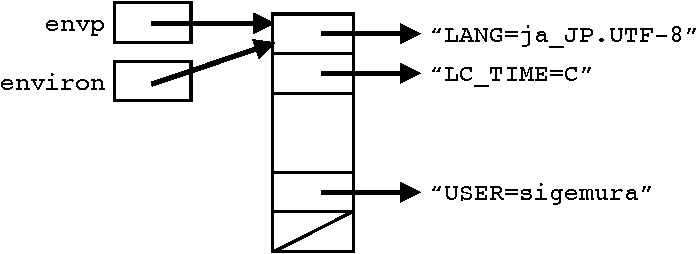
\includegraphics[scale=0.8]{Fig/environmentVariableData-crop.pdf}
    \end{myfig}

    \lstinputlisting[numbers=left
      %,caption=全ての環境変数を印刷するプログラム
      %,label=environmentVariablePrintAll
    ]{Lst/environmentVariablePrintAll.c}
  \end{description}

\item \emph{\texttt{getenv}関数を用いる.} \\
  \|getenv()|ライブラリ関数を用いて
  名前で指定した環境変数の値を読み出すことができる.

  \begin{description}
  \item [書式] \|getenv()|は次のような書式の関数である.

\begin{lstlisting}[numbers=none]
#include <stdlib.h>
char *getenv(char *name);
\end{lstlisting}

  \item [解説] \|name|には環境変数名を渡す.
    \|getenv()|は環境変数の値を表す文字列を指すポインタを返す.
    \|name|の環境変数が見つからない場合は\|NULL|ポインタを返す.

  \item [プログラム例]
    %リスト\ref{environmentVariablePrintLANG}のCプログラムは
    次のCプログラムは
    \|LANG|環境変数の値を表示するものである.
    4行で\|LANG|環境変数を探し,それの値(文字列)を指すポインタを返す.
    \|LANG|環境変数が見つかったら6行で\|LANG=|に続けて値を表示する
    (表示例は14行).
    見つからない場合は8行で見つからなかったことを意味するメッセージを表示する.

    \lstinputlisting[numbers=left
      %,caption=LANG環境変数の値を表示するプログラム,
      %,label=environmentVariablePrintLANG
    ]{Lst/environmentVariablePrintLANG.c}
  \end{description}
\end{enumerate}

\subsection{操作}
自プロセスのメモリ空間にコピーされた環境変数を操作する
三つのC言語ライブラリ関数を紹介する.
なお,一旦,環境変数を追加・変更・削除する操作を行うと
\|main()|の仮引数\|envp|は使用できなくなる(値がデタラメになる).
常にグローバル変数\|environ|を使用するとトラブルが少ない.

\begin{enumerate}
\item \emph{\texttt{setenv}関数} \\
  環境変数を新規に作成したり,値を上書きしたりする関数である.

  \begin{description}
  \item [書式] \|setenv()|は次のような書式の関数である.

\begin{lstlisting}[numbers=none]
#include <stdlib.h>
int setenv(char *name, char *val, int overwrite);
\end{lstlisting}

  \item [解説]
    \|name|は環境変数の名前,
    \|val|は環境変数にセットする値である.
    \|overwrite|は,\|0|の時に上書き禁止,
    それ以外の時に上書き許可を意味する.
    \|setenv()|は正常時に\|0|,エラー時に\|-1|を返す.
    上書き禁止の時,既に同じ名前の環境変数が存在するとエラーになる.
    エラー時は\|errno|大域変数にエラー番号がセットされる.

  \item [使用例] \|MYNAME|環境変数の値を\|sigemura|にする例を示す.
    第3引数が\|1|なので,
    \|MYNAME|環境変数が既に存在する場合は値の上書きになり,
    エラーにはならない.

\begin{lstlisting}[numbers=none]
setenv("MYNAME", "sigemura", 1);
\end{lstlisting}
  \end{description}

\item \emph{\texttt{putenv}関数} \\
  環境変数を新規に作成したり,値を上書きしたりする関数である.

  \begin{description}
  \item [書式] \|putenv()|は引数を一つだけ持つ.

\begin{lstlisting}[numbers=none]
#include <stdlib.h>
int putenv(char *string);
\end{lstlisting}

  \item [解説]
    \|string|は\|NAME=VALUE|形式の文字列である
    (それ以外の形式の文字列を渡すとエラーになる).
    \|putenv()|は正常時に\|0|,エラー時に\|-1|を返す.
    エラー時は\|errno|大域変数にエラー番号がセットされる.
    \|putenv("NAME=VALUE");|は,
    \|setenv("NAME","VALUE",1);|と同じ操作を行う.

  \item [使用例]
    前出の\|setenv()|の使用例と同じことを\|putenv()|を用いて行う例を示す.

\begin{lstlisting}[numbers=none]
putenv("MYNAME=sigemura");
\end{lstlisting}

  \item [注意]
    \|NAME=VALUE|形式の文字列を格納して\|putenv()|に渡した領域は,
    該当環境変数を記憶する領域として使い続けられる.
    この領域を書き換えたり,別の目的に再利用してはならない.

  \end{description}

\item \emph{\texttt{unsetenv}関数} \\
  環境変数を削除する関数である.

  \begin{description}
  \item [書式]  \|unsetenv()|も引数を一つだけ持つ.

\begin{lstlisting}[numbers=none]
#include <stdlib.h>
int unsetenv(char *name);
\end{lstlisting}

  \item [解説] \|name|は削除する環境変数の名前である.
    \|unsetenv()|は正常時に\|0|,エラー時に\|-1|を返す.
    エラー時は\|errno|大域変数にエラー番号がセットされる.

  \item [使用例] \|MYNAME|環境変数を削除する例を示す.

\begin{lstlisting}[numbers=none]
unsetenv("MYNAME");
\end{lstlisting}

  \end{description}
\end{enumerate}

%==============================================================================
\section*{課題 No.8}
\begin{enumerate}
\item 外部コマンドprintenvの仕様を調べる \\
  オンラインマニュアル(\|man 1 printenv|)を読んだり,
  \|printenv|を実際に実行したりして,
  printenvコマンドの仕様を調べなさい.
\item myprintenvプログラム\\
  外部コマンドprintenvと同様な働きをするmyprintenvプログラムを作成しなさい.
  なるべく本物と同じ動作をするように作ること.
\end{enumerate}
 
